\documentclass[
  captions=tableheading,
  bibliography=totoc, 
  titepage=firstiscover,
]{scrartcl}

\usepackage{blindtext} %neuer input

\usepackage{longtable} % Tabellen über mehrere Seiten

\usepackage[utf8]{inputenc} %neuer input

\usepackage{scrhack}

\usepackage[aux]{rerunfilecheck} %Warnung falls nochmal kompiliert werden muss

\usepackage{fontspec} %Fonteinstellungen

\recalctypearea{}

\usepackage[main=ngerman]{babel} %deutsche Spracheinstellung

\usepackage{ragged2e} %neuer input

\usepackage{amsmath, nccmath}

\usepackage{amssymb} %viele mathe Symbole

\usepackage{mathtools} %Erweiterungen für amsmath


\DeclarePairedDelimiter{\abs}{\lvert}{\rvert}
\DeclarePairedDelimiter{\norm}{\lVert}{\rVert}

\DeclarePairedDelimiter{\bra}{\langle}{\rvert}
\DeclarePairedDelimiter{\ket}{\lvert}{\rangle}

\DeclarePairedDelimiterX{\braket}[2]{\langle}{\rangle}{
#1 \delimsize| #2
}

\NewDocumentCommand \dif {m}
{
\mathinner{\symup{d} #1}
}


\usepackage[
  math-style=ISO,
  bold-style=ISO,
  sans-style=italic,
  nabla=upright,
  partial=upright,
  warnings-off={
    mathtools-colon,
    mathtools-overbracket,
  },
]{unicode-math}

\setmathfont{Latin Modern Math}
\setmathfont{XITS Math}[range={scr, bfscr}]
\setmathfont{XITS Math}[range={cal, bfcal}, StylisticSet=1]


\usepackage[
  locale=DE,
  separate-uncertainty=true,
  per-mode=reciprocal,
  output-decimal-marker={,},
]{siunitx}

\usepackage[autostyle]{csquotes} %richtige Anführungszeichen

\usepackage{xfrac}

\usepackage{float}

\floatplacement{figure}{htbp}

\floatplacement{table}{htbp}

\usepackage[ %floats innerhalb einer section halten
  section,   %floats innerhalb er section halten
  below,     %unterhalb der Section aber auf der selben Seite ist ok
]{placeins}

\usepackage[
  labelfont=bf,
  font=small,
  width=0.9\textwidth,
]{caption}

\usepackage{subcaption} %subfigure, subtable, subref

\usepackage{graphicx}

\usepackage{grffile}

\usepackage{booktabs}

\usepackage{microtype} %Verbesserungen am Schriftbild

\usepackage[
backend=biber,
]{biblatex}

\addbibresource{../lit.bib}

\usepackage[ %Hyperlinks im Dokument
  german,
  unicode,
  pdfusetitle,
  pdfcreator={},
  pdfproducer={},
]{hyperref}

\usepackage{bookmark}

\usepackage[shortcuts]{extdash}

%\usepackage{warpcol}

\usepackage{ulem}

\begin{document}
    \title{Physik IV Übungsblatt 2}
    \author{  
    Tobias Rücker\\
    \texorpdfstring{\href{mailto:tobias.ruecker@tu-dortmund.de}{tobias.ruecker@tu-dortmund.de}
    \and}{,} 
    Paul Störbrock\\
    \texorpdfstring{\href{mailto:paul.stoerbrock@tu-dortmund.de}{paul.stoerbrock@tu-dortmund.de}}{}
    }
\maketitle
\center{\Large Abgabegruppe: \textbf{4 H}}
\thispagestyle{empty}

\newpage
\tableofcontents
\thispagestyle{empty}
\newpage

\setcounter{page}{1}


\section{Aufagabe 1}

\begin{figure}[H]
    \centering
    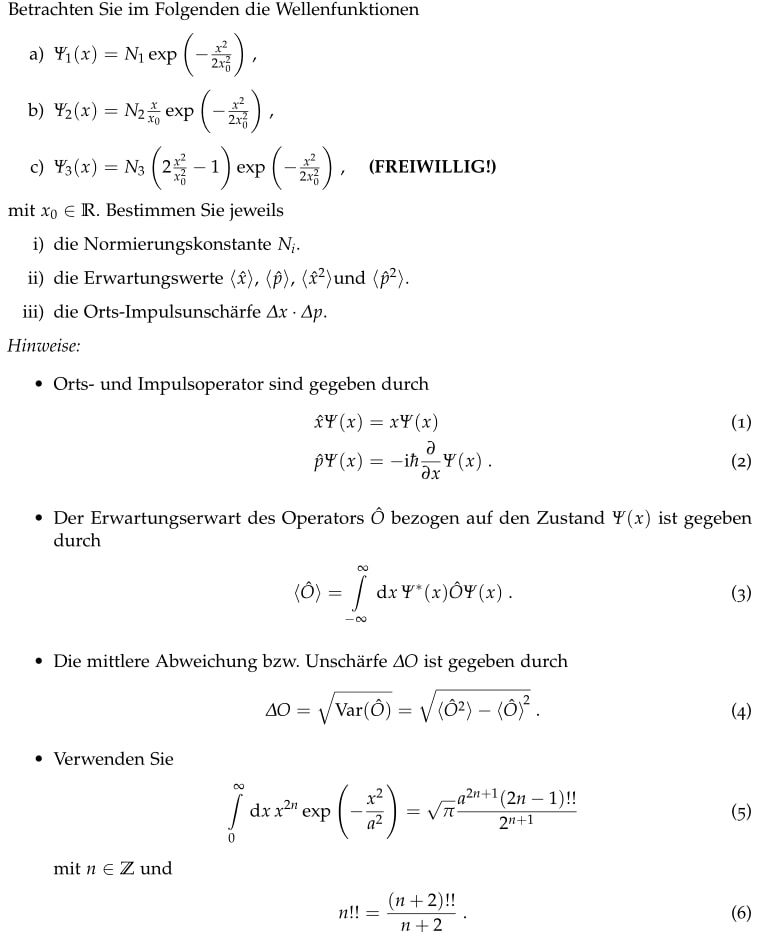
\includegraphics[width=0.75\textwidth]{images/Aufgabe_1.jpg}
    \label{fig:1}
\end{figure}

\subsection{a)}



\subsection{b)}



\subsection{c)}

\subsubsection{i)}

\subsubsection{ii)}

\subsubsection{iii)}



\section{Aufgabe 2}

\begin{figure}[H]
    \centering
    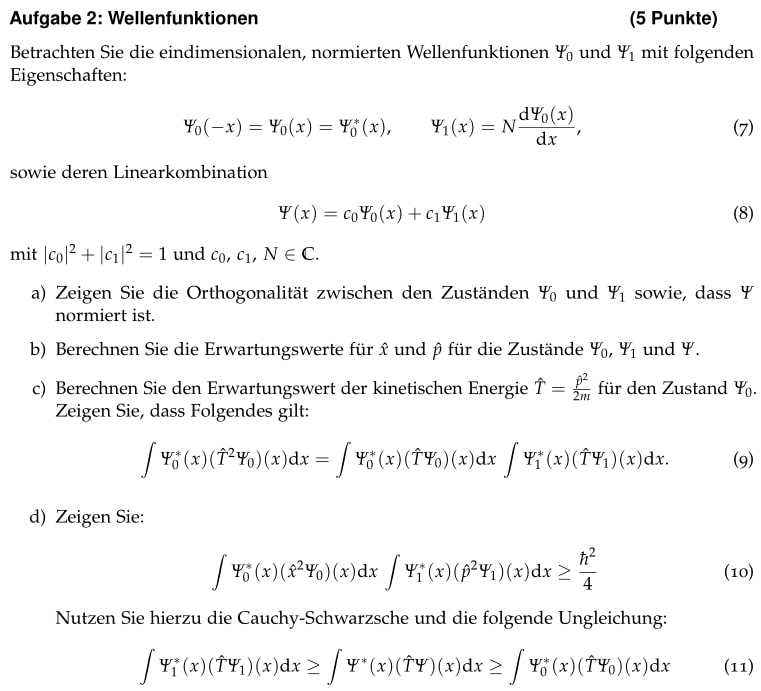
\includegraphics[width=0.75\textwidth]{images/Aufgabe_2.jpg}
    \label{fig:2}
\end{figure}

\subsection{a)}

\flushleft{Beweis\,}\justifying der Orthogonalität zwischen 
$\Psi _1 $ und $\Psi _2 $

Fall $\Psi _0 = \Psi _1$

\begin{align}
    <\Psi _0 , \Psi _0> &= \int_{-\infty}^{\infty} \,dx\, \Psi _0^* \Psi _0\\
    &= \int_{-\infty}^{\infty} \,dx\, \abs{\Psi _0 }^2 \\
    &=1
\end{align}

Beweis, dass $\Psi$ bereits normiert ist:



Fall: $\Psi _0 \ne \Psi _1$

\begin{align}
    <\Psi _0 , \Psi _1> &= \int_{-\infty}^{\infty} \,dx \, \Psi _0^* \cdot \Psi _1\\
    &=\int_{-\infty}^{\infty} \,dx\, \Psi _0 N \frac{d \Psi _0 (x)}{dx}\\
    &=\int_{-\infty}^{\infty} \,dx\, \frac{N}{2} \frac{d}{dx}(\Psi _0(x)\cdot \Psi _0(x))\\
    &=\frac{N}{2} \int_{-\infty}^{\infty} \,dx\,  \frac{d}{dx}(\Psi _0(x)\cdot \Psi _0^*(x))\\
    &=\frac{N}{2} \int_{-\infty}^{\infty} \,dx\, \frac{d}{dx}(\abs{\Psi _0(x)}^2)\\
    &=\frac{N}{2} [\abs{\Psi _0(x)}^2]_{-\infty}^ {\infty}
    \intertext{
        $\Psi _0 (x)$ ist gerade und läuft im Unendlichen gegen 0
        }
    \Rightarrow &= 0
\end{align}

\begin{align*}
    \mathrm{Z\kern-.3em\raise-0.5ex\hbox{Z}} \int_{-\infty}^{\infty} \, dx \, \abs{\Psi (x)}^2&=1\\
    \int_{-\infty}^{\infty} \, dx\, \abs{\Psi (x)}^2 &= \int_{-\infty}^{\infty}\, dx\, \abs{c_0 \Psi _0 (x) + c_1 \Psi _1(x)}^2\\
    &=\int_{-\infty}^{\infty} \, dx\, (c_0 \Psi _0  + c_1 \Psi _1)^* \,(c_0 \Psi _0  + c_1 \Psi _1)\\
    &=\int_{-\infty}^{\infty} \, dx\, (c_0^* \Psi _0  + c_1^* \Psi _1^*) \,(c_0 \Psi _0  + c_1 \Psi _1)\\
    &=\int_{-\infty}^{\infty} \, dx\, \abs{c_0}^2 \abs{\Psi _0}^2+\abs{c_1}^2 \abs{\Psi _1}^2 + c_0^* c_1 \Psi _0 \Psi _1+c_1^* c_0 \Psi _0 \Psi_1^*\\
    &=\int_{-\infty}^{\infty} \, dx\, \abs{c_0}^2 \abs{\Psi _0}^2 +\int_{-\infty}^{\infty} \, dx\,\abs{c_1}^2 \abs{\Psi _1}^2 +\int_{-\infty}^{\infty} \, dx\, c_0^* c_1 \Psi _0 \Psi _1+ \\
    &\phantom{=} \int_{-\infty}^{\infty} \, dx\, c_1^* c_0 \Psi _0 \Psi_1^*\\
    &= \abs{c_0}^2+\abs{c_1}^2+ \int_{-\infty}^ {\infty}\,dx\, \frac{c_0^*c_1}{N}\frac{1}{2} \frac{d}{dx}(\abs{\Psi _0}^2)+ \int_{-\infty}^{\infty} \,dx\, \frac{c_1^*c_0}{N^*}\frac{1}{2}\frac{d}{dx}(\abs{\Psi _0}^2) \\
    &= 1+ \underbrace{\left[\frac{c_0^*c_1}{2N}\abs{\Psi _0}^2\right]_{-\infty}^{\infty}}_{=0} + \underbrace{\left[\frac{c_1^*c_0}{2N^*}\abs{\Psi _0}^2 \right]_{-\infty}^{\infty}}_{=0} \\
    &=1
\end{align*}

\subsection{b)}



\subsection{c)}



\subsection{d)}



\section{Aufgabe 3}

\begin{figure}[H]
    \centering
    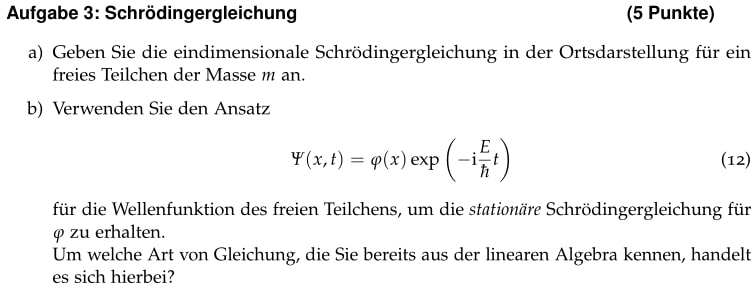
\includegraphics[width=0.75\textwidth]{images/Aufgabe_3ab.jpg}
    \label{fig:3}
\end{figure}

\subsection{a)}



\subsection{b)}



\begin{figure}[H]
    \centering
    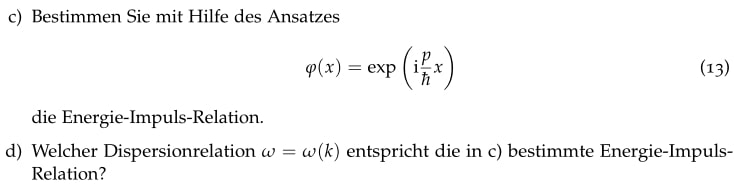
\includegraphics[width=0.75\textwidth]{images/Aufgabe_3cd.jpg}
    \label{fig:4}
\end{figure}

\subsection{c)}





\subsection{d)}



\end{document}